\documentclass{article}
\usepackage[utf8]{inputenc}
\usepackage[a4paper, portrait, margin=1in]{geometry}
\usepackage{graphicx}
\usepackage{amsmath}
\usepackage{amsfonts}
\usepackage{tabularx}
\usepackage{minted}
\usepackage{algorithmic}

\title{UE18CS342 \\Heterogeneous Parallelism \\Unit 1}
\author{Aronya Baksy}
\date{March 2021}

\begin{document}

\maketitle

\section{Introduction}
\begin{itemize}
    \item \textbf{Parallelism} involves connecting multiple processing units with an interconnection network, as well as the necessary software needed to coordinate these processing units. 
    
    \item The multiple processing units may all be the same (homogeneous) or may have different characteristics (heterogeneous)
    
    \item The two main types of hardware designs that acheive different goals are:
\end{itemize}

\subsection{Latency-Oriented Design}
\begin{itemize}
    \item In general, aim to execute as many instructions as possible belonging to a single serial thread, in a given window of time
        
    \item Some features of Latency Oriented Design are:
    \begin{enumerate}
        \item High clock frequency
            
        \item Large caches reduce the need for frequent memory accesses (that are high latency operations compared to cache access)
            
        \item Sophisitcated control logic includes features such as \textit{branch prediction}, \textit{predication}, \textit{fusion}, \textit{speculation} and \textit{data forwarding}
            
        \item Powerful and specialized ALUs for integer and floating point operations
    \end{enumerate}
\end{itemize}

\subsection{Throughput-Oriented Design}
\begin{itemize}
    \item Aim is to increase the throughput of the system, by parallelizing workloads.
        
    \item Some features of Throughput Oriented Design are:
    \begin{enumerate}
        \item Moderate clock frequency compared to latency-oriented designs
            
        \item Small caches, increasing the memory bandwidth utilization and the memory throughput
            
        \item Simpler control logic, no branch prediction and data forwarding hardware
            
        \item Energy-efficient and simple ALUs that are deeply pipelined for higher throughput.
            
        \item Require massive number of parallel operations to tolerate latencies
    \end{enumerate}
\end{itemize}

\subsection{Types of Parallelism}

\subsubsection{Bit-Level Parallelism}
\begin{itemize}
    \item Increasing processor word size, hence reduces number of instructions needed to process large data sizes (larger than word length)
    
    \item e.g.: An 8-bit processor will need 3 instructions to add 2 16-bit numbers but a 16-bit processor can do it in one instruction. 
\end{itemize}

\subsubsection{Instruction-Level Parallelism}
\begin{itemize}
    \item Concurrent execution of multiple instructions in the same stream. 
    
    \item Generated and managed by hardware (superscalar) or by compiler (VLIW)
    
    \item Limited in practice by data and control dependences
\end{itemize}

\subsubsection{Thread-Level Parallelism}
\begin{itemize}
    \item Multiple threads from the same application executed concurrently.
    
    \item Generated by the compiler, managed in hardware. 
    
    \item Limited in practice by communication/synchronization overheads and by algorithm characteristics
\end{itemize}

\subsubsection{Task-Level Parallelism}
\begin{itemize}
    \item Extraction of parallel tasks from control structures like \textbf{loops} and \textbf{functions}.
    
    \item A program exploiting loop-level parallelism uses multiple threads or processes which operate on some or all of the indices at the same time. 
    
    \item The speedup generated by such parallelism is in line with Amdahl's Law
\end{itemize}

\subsection{Flynn's Taxonomy}
\subsubsection{Single Instruction, Single Data}
\begin{itemize}
    \item Single control unit fetches single instruction stream from memory. The CU then generates appropriate control signals to direct single processing element to operate on single data stream i.e., one operation at a time.
    
    \item Can be classified as a serial scalar computer. 
    
    \item e.g.: Intel 4004
\end{itemize}

\subsubsection{Single Instruction, Multiple Data}
\begin{itemize}
    \item A single instruction executes on multiple data streams. 
    
    \item A single operation on a vector can be thought of as applying the same instruction stream to each element of the vector (each element being a data stream)
    
    \item Instructions can be executed in sequence (using pipelining) or in parallel (with multiple functional units). 
    
    \item e.g.: CRAY-1, ICL DAP
\end{itemize}

\subsubsection{Multiple Instruction, Single Data}
\begin{itemize}
    \item Multiple instructions operate on one data stream. 
    
    \item This is an uncommon architecture which is generally used for fault tolerance.
    
    \item e.g.: Space Shuttle flight computer, Colossus Mark II
\end{itemize}

\subsubsection{Multiple Instruction, Multiple Data}
\begin{itemize}
    \item Multiple autonomous processors simultaneously executing different instructions on different data. 
    
    \item e.g.: Multi processors and Multi computers
\end{itemize}

\begin{figure}[!t]
    \centering
    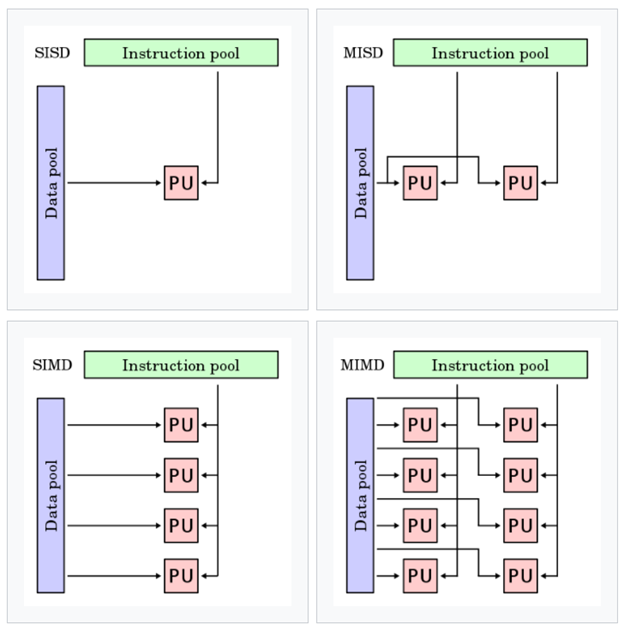
\includegraphics[scale=0.5]{flynn.png}
    \caption{Flynn's Taxonomy}
    \label{fig:my_label}
\end{figure}

\section{ILP Enhancement Techniques}
\begin{itemize}
    \item CPU performance is dependent on three factors as shown in the below equation:
    \begin{equation*}
        T_{CPU} = Instr \times CPI \times t_{cycle}
    \end{equation*}
    
    \item Improvement in CPU performance involves either
    \begin{itemize}
        \item Reducing number of executed instructions (with better algorithms, compiler optimizations or better ISAs)
    
        \item Reducing the cycle time (depends on technology, organization and logic design). Increasing clock speed is a solution but only till a physical limit
        
        \item Reducing the CPI (introducing more overlap between instructions, depends on the ISA and the CPU organization). The key is \textbf{parallelism} (at instruction level using pipelining, or internally using superscalar processors with multiple functional units or multiple cores, or externally using multiple CPUs)
    \end{itemize} 
    
    \item Average CPI is calculated as
    \begin{equation*}
        CPI = \sum_{i=1}^{n} F_i \times CPI_i
    \end{equation*}
    
    where $F_i$ is the probability of encountering instruction of type $i$ having CPI equal to $CPI_i$
    
    \item Hazards prevent the next instruction in the instruction stream from being executing during its designated clock cycle.
    
    \item Hazards reduce the performance from the ideal speedup gained by pipelining.
    
    \item Types of hazards:
    \begin{itemize}
        \item \textbf{Structural Hazards}: Resource conflicts when the hardware cannot support all possible combinations of instructions in simultaneous overlapped execution.
        
        \item \textbf{Data Hazards}: Instruction depends on the result of a previous instruction in a way that is exposed by the overlapping of instructions in the pipeline. (e.g.: WAW, WAR, RAW)
        
        \item \textbf{Control Hazards}: Arise from pipelining of branches and other instructions that change the PC.
    \end{itemize}
\end{itemize}

\subsection{Dependencies}
\begin{itemize}
    \item Dependencies are artifacts of programs while hazards are artifacts of pipeline architecture and organization
    
    \item Not all dependencies translate directly into pipeline hazards
    
    \item Software approaches to handle dependencies are:
    \begin{enumerate}
        \item Reorder instructions at compile time
        
        \item Insert no-op instructions
        
        \item Loop unrolling
    \end{enumerate}
\end{itemize}

\subsubsection{Data Dependencies}
\begin{itemize}
    \item Also called \textit{true dependencies}
    
    \item Let instruction $i$ occur before instruction $j$ in the execution order. $j$ is said to be data dependent on $i$ if
    \begin{itemize}
        \item $j$ may use a result that is produced by $i$
        
        \item $j$ is dependent on instruction $k$ and $k$ is dependent on $i$
    \end{itemize}
\end{itemize}

\subsubsection{Name Dependencies}
\begin{itemize}
    \item When 2 instructions use the same name (i.e. register name) but there is no data flow between the instructions. 
    
    \item Let instruction $i$ occur before instruction $j$ in the execution order:
    \begin{itemize}
        \item An \textbf{anti-dependency} arises when $j$ writes to a location that is read by $i$
        
        \item An \textbf{output dependency} arises when both $i$ and $j$ write to the same register or memory location
    \end{itemize}
    
    \item If the dependencies can be removed (using register renaming maybe) then such instructions \textit{can} be parallelized
\end{itemize}

\subsubsection{Control Dependencies}
\begin{itemize}
    \item Dependency of instructions to the sequential flow of execution and preserves flow-altering behavior of the program (such as branching)
    
    \item Two types of constraints:
    \begin{itemize}
        \item An instruction that is control-dependent on a branch cannot be moved before the branch to make it control independent
        
        \item An instruction that is control-independent of the branch cannot be moved after the branch to make it dependent on the branch
    \end{itemize}
\end{itemize}

\subsection{Dynamic Scheduling: Tomasulo's Algorithm}
\begin{itemize}
    \item This involves designing hardware that can reorder instructions at runtime while preserving data flow and exception behaviour
    
    \item Advantages of dynamic scheduling:
    \begin{itemize}
        \item Simplifies the compiler as it no longer has to take care of reordering instructions
        
        \item Allows instructions compiled for one pipeline to run on other pipelines efficiently as well
    \end{itemize}
    
    \item Dynamic scheduling is implemented either as \textbf{scoreboarding} or using \textbf{Tomasulo's Algorithm}. 
    
    \item In-order issue of instructions, but out-of-order execution (which leads to out-of-order completion).
    
    \item Register renaming is used by Tomasulo's Algorithm to correctly perform OO execution. 
     
    \item Out-of-order completion leads to WAR/WAW data hazards, as well as complications in exception handling 
\end{itemize}

\subsubsection{Components of Tomasulo's Organization}
\begin{itemize}
    \item \textbf{Reservation Station}: 
    \begin{itemize}
        \item Allow the CPU to make use of a value as soon as it has been computed instead of waiting for it to be written to a register and reading from there
        
        \item It checks if the operands are available (avoid RAW) and if execution unit is free (avoid Structural hazard) before starting execution.
        
        \item Instructions are stored with available parameters, and executed when ready. 
        
        \item Results are identified by the unit that will execute the corresponding instruction. Implicitly \textit{register renaming} solves WAR and WAW hazards.
    \end{itemize}
    
    \item Registers in instructions are replaced with pointers to the reservation stations that will produce those values. This act is called \textit{register renaming}. 
    
    \item As there are more reservation stations than there are registers, it allows for optimizations that compilers cannot do, as well as elimiation of WAR and WAW hazards. 
    
    \item Instructions are issued in sequence to Reservation Stations which buffer the instruction as well as the operands of the instruction.
    
    \item If the operand is not available, the Reservation Station listens on a \textbf{Common Data Bus} for the operand to become available. When the operand becomes available, the Reservation Station buffers it, and the execution of the instruction can begin.

    \item Functional Units (e.g.: FP Adder, FP multiplier), each have their corresponding Reservation Station. The output of the Functional Unit connects to the Common Data Bus, where Reservation Stations are listening for the operands they need.
    
    \item The data values stored in a Reservation Station are:
    \begin{itemize}
        \item \textbf{Op}: The operand (ADD, SUB, MUL, DIV, etc.) for the instruction
        
        \item $V_j, V_k$: The actual register \textbf{values} (i.e. values of the source operands) are stored here
        
        \item $Q_j, Q_k$: The reservation station that will produce the relevant source operand, in case it is not yet available (A value of 0 indicates that the relevant result is already in one of the $V$ fields)
        
        \item \textbf{Busy}: Indicates whether that station is currently busy or not. 
    \end{itemize}
    
    \item \textbf{Load/Store Buffers} maintain 2 fields, a busy bit (indicating whether that buffer entry is full or not) and the memory address to be loaded. 
\end{itemize}

\subsubsection{Tomasulo's Algorithm Stages}
\begin{enumerate}
    \item \textbf{Issue}: get instruction from FP operation queue. If a reservation station is free then the control issues the instruction and sends the operands.
    
    \item \textbf{Execute}: Watch CDB to pick up operands from prior instructions. When both operands ready, can execute
    
    \item \textbf{Write Back}: Write to all waiting units via CDB, and mark the reservation station as free
\end{enumerate}

\subsubsection{Drawbacks of Tomasulo's Algorithm}
\begin{itemize}
    \item High complexity of the hardware and control logic
    
    \item Many associative stores (CDB) at high speed
    
    \item The CDB speed is a bottleneck on the performance of the algorithm. If each CDB must reach multiple functional units, it implies high capacitance and high wiring density (which ofc leads to higher heat dissipation)
    
    \item Only one functional unit can complete execution in each cycle. For multiple FUs to complete at once, more CDBs are needed, which means extra control logic for parallel associative stores
    
    \item Imprecise exceptions (exceptions wherein the processor cannot restart directly from the point where the exception was thrown) cannot be handled.
\end{itemize}

\section{Speculative Execution}
\begin{itemize}
    \item Speculative execution is an optimization technique where the CPU executes an instruction before it is known whether it is actually needed.
    
    \item This is done so as to prevent a delay that would have to be incurred by executing the instruction after it is known that it is needed. 
    
    \item If it turns out the instruction's result was not needed after all, most changes made by the instruction are reverted and the results are ignored.
\end{itemize}
\subsection{Hardware Support for Precise exceptions}
\begin{itemize}
    \item A \textit{reorder buffer} allows instructions to be committed in-order.
    
    \item An extra \textbf{Commit} stage is added to the Tomasulo Algorithm. 
    
    \item  In this stage, the results of instructions will be stored in a register or memory. In the "Write Result" stage, the results are just put in the re-order buffer. All contents in this buffer can then be used when executing other instructions depending on these.
\end{itemize}

\subsection{Tomasulo's Algorithm Stages}
\begin{itemize}
    \item \textbf{Issue}: get instruction from FP op queue. If reservation station \textbf{and} reorder buffer slot are free, issue instr, send operands and reorder buffer no.
    
    \item \textbf{Execution}: When both operands ready then execute. If not ready, watch CDB for result. When both in reservation station, execute

    \item \textbf{Write Result}: Write on Common Data Bus to all awaiting FUs and reorder buffer. Mark reservation station available.
    
    \item \textbf{Commit}: update register with reorder result. When instr. at head of reorder buffer \& result present, update register with result (or store to memory) and remove instr from reorder buffer. A mispredicted branch flushes the reorder buffer
\end{itemize}

\begin{tabular}{|p{0.45\linewidth}|p{0.45\linewidth}|}
    \hline
    \textbf{Hardware Speculatio} & \textbf{Software Speculation}  \\
    \hline
    Runtime memory disambiguation done using Tomasulo's Algorithm, allows loads to move past stores at runtime & Runtime memory disambiguation is difficult at compile time when pointers are involved \\
    \hline
    Works better when control flow is not predictable & Hardware branch pred beats software branch pred that is done at compile time \\
    \hline 
    Maintains completely precise execution model even for speculated instructions & Need added spl support for this in software \\
    \hline
    Do not require compensation or bookkeeping code & Compensation and bookkeeping are needed \\
    \hline 
    Lookahead in code is limited & Better possible scheduling due to the ability to see the entire code at compile time \\
    \hline
\end{tabular}


\subsection{Thread-Level Speculation}
\begin{itemize}
    \item Speculative execution of a sequence of code that is anticipated to be executed in parallel on an independent thread
    
    \item Assumptions need to be made about input values. If assumptions are correct then thread can run faster
    
    \item If assumptions are wrong then thread needs to be squashed and discarded. 
    
    \item TLS allows the compiler to optimistically create threads at runtime despite ambiguity about data dependencies, as well as detect such violations and recover from them at runtime. 
\end{itemize}



\section{Predicative Execution}
\begin{itemize}
    \item Associate a Boolean expression (i.e. a predicate) with the issue/execution/commit of an instruction
    
    \item The result of the instruction is either retained or invalidated depending on whether the predicate evaluates to a Boolean true or a Boolean false. 
    
    \item In \textbf{partial predication}, only a few specific opcodes have predicates associated with them. In \textbf{full predication}, all instructions are predicated.
    
    \item Central idea behind predication is that the compiler converts control dependence into data dependence, meaning that branch is eliminated (allows for sequential execution rather than changes in control flow)
    
    \item Advantages of predcation:
    \begin{itemize}
        \item Eliminate mis-predictions for hard-to-predict branches
        
        \item Reduce number of branches tested per cycle
        
        \item When misprediction cost is larger than the cost for doing useless work, predication works very well
        
        \item Instructions can be freely reordered without regard for any control dependencies
    \end{itemize}
    
    \item Disadvantages of predication:
    \begin{itemize}
        \item Increased fetch utilization, increased register consumption
        
        \item Easy-to-predict branches become costly due to extra useless work
        
        \item Static predication is not adaptive to run-time branch behavior.
        
        \item Increased FU utilization if predicates are tested at commit time
        
        \item All hard-to-predict branches (such as loop branches) are not completely eliminated
        
        \item Additional hardware and ISA support, larger instruction cache needed. 
    \end{itemize}
\end{itemize}

\section{Dependency Analysis}
\subsection{Types of Dependencies}
\begin{itemize}
    \item \textbf{True Dependency}: Instruction $S_i$ precedes instruction $S_j$, and instruction $S_i$ computes a value that is used by $S_i$. This means that $S_i$ \textbf{must} execute before $S_j$
    
    \item True dependency in the above example is denoted as $S_i\text{ }\delta^+\text{ }S_j$
    
    \item \textbf{Anti Dependency}: Instruction $S_i$ precedes instruction $S_j$, and instruction $S_i$ uses a value that is computed by $S_i$. This means that $S_i$ \textbf{must} execute before $S_j$
    
    \item Anti dependency is denoted as $S_i\text{ }\delta^a\text{ }S_j$
    
    \item \textbf{Output Dependency}: Instruction $S_i$ precedes instruction $S_j$, and instruction $S_i$ computes a value that is also computed by $S_i$. This means that $S_i$ \textbf{must} execute before $S_j$
    
    \item Output dependency is denoted as $S_i\text{ }\delta^o\text{ }S_j$
    
    \item \textbf{Input Dependency}: Instruction $S_i$ precedes instruction $S_j$, and instruction $S_i$ uses a value that is also used by $S_i$. \textbf{Not necessary} that $S_i$ must execute before $S_j$
    
    \item Input dependency is denoted as $S_i\text{ }\delta^I\text{ }S_j$
    
    \item Every dependency except true dependency can be eliminated using renaming. 
\end{itemize}

\subsection{Iteration Space}
\begin{itemize}
    \item Iteration space is the set of iterations , whose ID’s are given by the values held by the loop index variables
    
    \item e.g.: the iteration space for the loop
    
    \begin{minted}{c}
        for(int i=2; i<100; i = i+3)
        {
            z[i] = 0;
        }
    \end{minted}
    
    is the set $\{2, 5, 8, 11, ..., 95, 98\}$
    
    \item The \textit{normalized iteration space} is given as:
    \begin{equation*}
        i_n = \frac{i-i_{min}}{step}\text{ }\forall\text{ }i\text{ }\in\text{ }IterSpace
    \end{equation*}
\end{itemize}

\subsection{Dependence Testing}
\begin{itemize}
    \item Given the loop below:
    \begin{minted}{c}
        for (i in IterSpace1)
        {
            for(j in IterSpace2)
            {
                a[f(i, j)] = expr1;
                expr2 = a[g(i, j)];
            }
        }
    \end{minted}
    
    \item A dependence is said to exist if there exist 2 iteration vectors $\overrightarrow{k}, \overrightarrow{j}$ such that $f(\overrightarrow{k}) = g(\overrightarrow{j})$
    
    \item An algorithm that reports dependence only when one exists is called an \textbf{exact dependence test}. Else it is called an \textbf{in-exact dependence test}.
    
    \item Dependence tests must be conservative: if dependence cannot be ascertained, the test must still report that a dependence exists
    
    \item NOTE: The equation $a_1 i_1 + a_2 i_2 + a_3 i_3 + ... + a_n i_n = c$ has a solution only if $c$ is divisible exactly by $gcd(a_1, a_2, a_3, ..., a_n)$. This form of linear equation is called a \textbf{Diophantine Equation}.
\end{itemize}

\subsubsection{Affine Array Access}
\begin{itemize}
    \item Every array access can be formulated as a matrix equation. Given a loop of length $d$, the iteration space is represented as 
    \begin{equation*}
        \{ i \in \mathbb{Z}^d | Bi + b \ge 0 \}
    \end{equation*}
    
    Where $B$ is a $d \times d$ matrix, $b$ is a vector of length $d$ and 0 is a zero vector of length $d$. 
    
    \item e.g.: For the loop:
    \begin{minted}{c}
        for(i = 0; i <= 5; ++i)
            for(j=1; j<=7; ++j)
                z[j, i] = 0;
    \end{minted}
    
    we have the following:
    \begin{align*}
        i \ge 0 &\implies i + 0j + 0\ge 0 \\
        i \le 5 &\implies -i + 0j +5 \ge 0 \\
        j \ge 1 &\implies 0i + j - 1 \ge 0 \\
        j \le 7 &\implies 0i -j + 7 \ge 0
    \end{align*}
    
    \item An array access is called Affine if the bounds of the loop and the index of each dimension of the array are affine expressions of loop variables and symbolic constants
    
    \item Affine accesses can be represented as linear equations (matrix-vector equations)
    
    \item Affine functions map from iteration space to data space, hence easier to identify iterations that map to the same data. 
\end{itemize}

\subsection{Indices and Subscripts}
\begin{itemize}
    \item An index is a variable that appears in a subscript of an array (commonly denoted as $i, j, k ...$)
    
    \item A subscript is the set of all expressions that occur at one particular position within an array access. (e.g.: in the expression $A[i, j] = A[i, k] + c$ the first subscript is the set $\{i, i\}$ and the second subscript is the set $\{j, k\}$
    
    \item A subscript is said to be a:
    \begin{enumerate}
        \item \textbf{Zero Index Variable} if it contains no index variables
        
        \item \textbf{Single Index variable} if it contains exactly one index variable
        
        \item \textbf{Multiple Index Variable} if it contains more than 1 index variable
    \end{enumerate}
    
    \item e.g.: The expression $A(5, i+1, j) = A(1, i, k) + c$ contains the subscripts $\{5, 1\}$ (zero index), $\{i+1, i\}$ (single index) and $\{j, k\}$ (multiple index)
    
    \item Two subscripts are said to be \textbf{coupled} if the index variables appearing in one subscript also appear in the other. 
    
    \item Two subscripts that are not coupled are called \textbf{separable}
\end{itemize}

\subsection{Conservative Testing}
\begin{itemize}
    \item Considers only linear subscript expressions, tries to assert that "no dependence exists between 2 subscript expressions of one array reference"
    
    \item It is never incorrect (as it is conservative) but it is sub-optimal
    
    \item Partition subscripts into separable and minimally coupled groups. 
    
    \item For separable subscripts, apply single subscript tests. For coupled groups apply multi-subscript tests like the Delta test.
\end{itemize}
\subsection{Delta Test}
\begin{itemize}
    \item Let the source iteration be denoted as $I_0$ and the sink iteration denoted as $I_0 + \Delta I$. Solve the equation $f(I_0) = g(I_0 + \Delta I)$
    
    \item For the expression $A(i+1) = A(i) + B$ we have $I_0 +1 = I_0 + \Delta I$, which yields $\Delta I = 1$. Hence the distance vector is $(1)$ and the direction is $(+)$
    
    \item For the expression $A(i+1, j, k) = A(i, j, k+1) + B$ we have the equations
    \begin{align*}
        I_0 + 1 &= I_0 + \Delta I \\
        J_0 &= J_0 + \Delta J\\
        K_0 &= K_0 + \Delta K + 1
    \end{align*}
    
    which give $\Delta I = 1, \Delta J = 0, \Delta K = -1$. Hence the distance vector is $(1, 0, 1)$ with directions $(+, 0, -)$
    
    \item For the expression $A(i+1) = A(i) + B(j)$ we have $I_0 + 1 = I_0 + \Delta I$ which gives $\Delta I = 1$. Since $j$ has no source, its direction is unconstrained. The distance vector is given as $(+1, *)$
\end{itemize}

\subsection{Challenges of Dependency testing}
\begin{itemize}
    \item Unknown loop bounds can lead to false dependences
    \item Need to be conservative about aliasing
    \item Triangular loops and new constraints
\end{itemize}
\end{document}
